\documentclass[bachelor]{HDU-Bachelor-Thesis}

\usepackage{float}
\graphicspath{{thesis_figures/}}

\begin{document}

\pagenumbering{plain}
\pagestyle{plain}

% -------------------- 封面 --------------------
\thispagestyle{empty}
\begin{center}
\vspace*{2cm}
{\hei\zihao{1}\textbf{杭州电子科技大学}\par}
\vspace{1.5cm}
{\hei\zihao{-1}\textbf{本科毕业设计（论文）}\par}
\vspace{2cm}
{\song\zihao{2}题目：基于提示词优化的细粒度猫狗分类方法研究\par}
\vspace{3cm}
\begin{tabular}{l@{\hspace{3cm}}l}
\textbf{学院} & \underline{\hspace{5cm}} \\
\textbf{专业} & \underline{\hspace{5cm}} \\
\textbf{学号} & \underline{\hspace{5cm}} \\
\textbf{姓名} & \underline{\hspace{5cm}} \\
\textbf{指导教师} & \underline{\hspace{5cm}} \\
\end{tabular}
\vspace{2cm}
{\song\zihao{4}2026年5月\par}
\end{center}
\pagebreak

% -------------------- 前置部分 --------------------
\pagestyle{plain}
\pagenumbering{Roman}
\begin{abstract}

细粒度图像分类要求模型在同一大类内部区分视觉差异很小的子类,典型任务包括鸟类、车型和宠物品种识别。与普通图像分类相比,该任务往往面临类间差异小、类内变化大的问题,在少样本条件下尤其容易出现特征不足和类别混淆。Oxford-IIIT Pets 数据集中的猫狗品种识别就具有这一特点: 不同品种在毛色、脸型和体态上只存在局部差别,而拍摄姿态、光照和遮挡又会进一步干扰分类。

视觉语言预训练模型 CLIP 为小样本图像分类提供了新的实现路径。它可以利用图像与文本的对齐能力完成零样本或少样本识别,但分类效果仍然明显依赖提示词设计。已有的 CoOp 通过学习上下文向量替代人工提示词,改善了下游任务适配能力; CoCoOp 进一步引入图像条件化提示,提高了不同样本之间的适应性。不过,这两类方法都没有直接区分易分类样本和难分类样本,训练时仍采用统一的损失权重。

针对上述问题,本文提出一种基于 CoCoOp 的难样本加权扩展方法,并在项目中以 DynamicPromptTrainer 训练器形式实现。该方法以 CLIP 为基础,沿用可学习上下文和图像条件提示机制生成动态提示,并进一步引入难度权重计算器,根据模型对真实类别的预测置信度和错误情况生成可学习的样本权重,使训练过程对困难样本给予更高关注。与此同时,本文采用随 shot 数变化的自适应训练轮数策略,以缓解低样本条件下训练不足和高样本条件下过拟合的问题。

本文在 Oxford-IIIT Pets 数据集上完成了 1-shot、2-shot、4-shot、8-shot 和 16-shot 五组实验。结果表明,所提方法在 2-shot、4-shot、8-shot 和 16-shot 设置下均优于 CoCoOp,对应准确率分别达到 85.9\%、89.5\%、89.2\% 和 89.8\%; 其中 16-shot 设置下取得全实验最高准确率 89.8\%。实验结果说明,将图像条件提示与难度感知加权结合起来,能够更稳定地提升 CLIP 在细粒度少样本分类任务中的表现。

\keywords{细粒度分类,CLIP,提示词学习,少样本学习,猫狗品种识别}

\end{abstract}

\begin{abstractEN}

Fine-grained image classification aims to distinguish subcategories within the same coarse category, where visual differences are subtle and intra-class variation is often large. Pet breed recognition on Oxford-IIIT Pets is a typical example: breeds may differ only in local traits such as fur pattern, face shape, or body proportion, while pose, lighting, and occlusion still introduce strong appearance changes. These factors make the task difficult under few-shot supervision.

CLIP provides a practical foundation for this setting because it aligns image and text representations in a shared space. Yet its performance is still sensitive to prompt design. CoOp improves task adaptation by replacing handcrafted context words with learnable vectors, and CoCoOp further introduces image-conditional prompts. However, these methods do not explicitly distinguish easy samples from hard ones during training, and all samples still contribute to the loss in a similar manner.

This thesis presents a hard-sample weighting extension built on top of CoCoOp for fine-grained cat and dog classification, implemented in the project through the trainer named DynamicPromptTrainer. Built on CLIP, the method keeps the learnable context and image-conditional prompting scheme, and further introduces a difficulty weight calculator to assign learnable sample weights according to prediction confidence and misclassification status. In addition, an adaptive epoch schedule is adopted so that lower-shot settings receive longer training while higher-shot settings avoid unnecessary overfitting.

Experiments are conducted on the Oxford-IIIT Pets dataset with five few-shot settings: 1-shot, 2-shot, 4-shot, 8-shot, and 16-shot. The proposed method achieves 85.9\%, 89.5\%, 89.2\%, and 89.8\% accuracy in the 2-shot, 4-shot, 8-shot, and 16-shot settings, respectively, outperforming CoCoOp in all four cases. The best result reaches 89.8\% under the 16-shot setting. These results show that combining image-conditioned prompts with difficulty-aware weighting is effective for improving CLIP-based fine-grained few-shot classification.

\keywordsEN{Fine-grained Classification, CLIP, Prompt Learning, Few-shot Learning, Pet Breed Recognition}
\end{abstractEN}


\tableofcontents
\pagebreak

% -------------------- 正文 --------------------
\pagenumbering{arabic}
\chapter{绪论}

\section{研究背景与意义}

细粒度图像分类关注的不是“大类是否正确”,而是同一大类内部的子类区分。例如,普通分类任务只需判断图像是猫还是狗,细粒度分类则要求继续识别英短、布偶、暹罗、柴犬、哈士奇等具体品种。与粗粒度分类相比,该任务通常同时具有类间差异小和类内变化大的特点: 不同类别之间可能只在耳朵形状、毛发纹理、脸部轮廓或体态比例上存在局部差别,而同一类别又会因为姿态、光照、背景和遮挡的变化呈现出明显不同的外观\cite{parkhi2012cats,atabuzzaman2025zero}。这使得细粒度分类对模型的特征表达能力提出了更高要求。

从模型发展过程来看,深度学习显著推动了图像分类性能提升。AlexNet 在 ImageNet 上取得突破后,卷积神经网络开始成为视觉任务的基础方案\cite{krizhevsky2012imagenet}。随后,VGG 和 ResNet 等结构进一步改善了模型深度和训练稳定性\cite{simonyan2015very,he2016deep}。这些方法在标准分类任务上取得了很强的效果,但它们通常建立在大量标注数据的基础上。对于细粒度任务而言,高质量标注往往更难获取,一方面是因为类别数较多,另一方面是因为部分类别之间需要较强的领域知识才能准确区分。

宠物品种识别就是一个很典型的例子。Oxford-IIIT Pets 数据集包含 37 个猫狗品种,图像数量有限,并且样本在姿态、尺度、背景和拍摄质量上变化明显\cite{parkhi2012cats,oxfordpetsweb}。已有研究表明,即使是犬种分类这样接近日常应用的任务,卷积网络在面对外观相近类别时仍然容易产生混淆\cite{cuizhang2023classification}; 对于猫类识别,细粒度差异通常更依赖局部特征,迁移学习与分层特征利用才可能取得更稳定的结果\cite{wang2024enhancing}。因此,围绕宠物品种展开细粒度分类研究,不仅具有明确的实验价值,也具备实际应用意义。

近年来,视觉语言预训练模型为小样本视觉任务提供了新的技术路径。CLIP 通过大规模图文对比学习建立了统一的图像和文本语义空间,使模型可以借助文本提示完成零样本分类\cite{clip2021}。与传统分类网络相比,它不需要为每个任务单独训练完整分类头,在标注数据有限的场景下具有明显优势。不过,CLIP 在下游任务中的表现对提示词设计高度敏感。对于细粒度类别,如果提示词过于通用,文本语义往往不足以支撑不同品种之间的细微区分。

围绕这一问题,提示学习逐渐成为视觉语言模型适配的重要方向\cite{gu2023prompt,chen2023vlp}。研究者开始尝试用可学习上下文替代人工模板,并进一步引入图像条件提示和细粒度多模态提示,以改善 CLIP 在少样本场景中的表现\cite{coop2022,cocoop2022,liu2025fgmpl}。这说明提示词已经不再只是输入文本的修饰,而逐渐成为模型适配策略本身的一部分。

本文的工作正是在这一背景下展开。研究重点是: 在 Oxford-IIIT Pets 数据集的少样本设置下,如何通过动态提示优化提高 CLIP 对细粒度猫狗品种的分类能力。相比于直接微调整个模型,提示学习参数量更小,训练成本更低,也更适合本科毕业设计的实验条件; 相比于固定模板,动态提示则更有可能适应不同图像和不同分类难度的样本。

\section{国内外研究现状}

\subsection{细粒度图像分类研究}

细粒度分类并不是随着大模型才出现的研究方向。早期方法更多依赖人工设计特征、部件检测和属性建模,希望通过局部区域或相对属性来刻画子类别之间的差异。Oxford-IIIT Pets 数据集提出时,研究者就已经把宠物品种识别视作细粒度视觉识别问题,并指出该任务对局部形状和毛发表观建模提出了较高要求\cite{parkhi2012cats}。这类方法有助于解释模型关注了哪些区域,但往往依赖较强的任务先验和人工特征设计。

深度学习兴起后,细粒度分类逐渐转向端到端特征学习。卷积神经网络凭借层级表示能力,在鸟类、车辆和宠物等任务上取得了更稳定的结果。围绕宠物分类,已有研究尝试采用卷积网络结合传统分类器实现犬种识别,结果表明类别相似性和样本复杂度仍然是限制性能的重要因素\cite{cuizhang2023classification}。也有工作从迁移学习角度改进细粒度猫类识别,说明对中高层特征进行更细致的利用能够带来性能提升\cite{wang2024enhancing}。

随着视觉语言模型的发展,细粒度分类又出现了新的切入点。Atabuzzaman 等人在 EMNLP 2025 Findings 中讨论了大规模视觉语言模型在零样本细粒度分类上的潜力,指出更合理的类别描述和提示设计能够显著影响模型表现\cite{atabuzzaman2025zero}。这一结果说明,语言信息并不是附属输入,在细粒度任务中反而可能成为增强类别区分能力的重要补充。

\subsection{视觉语言预训练与提示学习研究}

CLIP 的提出使视觉语言预训练成为当前多模态研究的重要基础\cite{clip2021}。该模型通过大规模图文对学习跨模态对齐表示,图像特征和文本特征被映射到同一语义空间中,从而可以通过文本模板直接完成分类。围绕视觉语言预训练,后续研究和综述逐渐形成较为完整的知识框架。Chen 等人的综述系统梳理了视觉语言预训练的模型结构、训练目标和下游任务\cite{chen2023vlp}; Gu 等人则从提示工程角度总结了视觉语言基础模型中的提示形式与应用场景\cite{gu2023prompt}。这些工作都表明,提示已经成为视觉语言模型适配不可回避的核心问题。

在具体方法上,CoOp 是视觉任务提示学习的代表工作\cite{coop2022}。它将人工文本模板中的上下文词替换为可学习向量,并利用少量下游样本优化这些向量,从而使提示更符合目标数据集分布。CoOp 的关键贡献在于证明了一个事实: 在很多任务中,无需微调整个视觉编码器,只通过学习少量提示参数就可以显著提升 CLIP 的分类性能。

不过,CoOp 的提示是静态共享的,所有图像都使用同一组上下文向量。当任务内部样本变化较大时,这种统一提示很难同时适应所有输入。为此,Zhou 等人进一步提出 CoCoOp,在静态提示基础上增加图像条件 token,使不同图像能够获得不同的提示偏移\cite{cocoop2022}。CoCoOp 把提示学习从任务级共享推进到样本级适配,在少样本泛化和跨数据集测试中表现出更好的鲁棒性。

在 CoOp 和 CoCoOp 之后,提示学习开始向更复杂的方向发展。一类工作关注自动提示优化。ProAPO 通过渐进式策略对提示进行自动搜索和改进,以减少手工设计的参与程度\cite{qu2025proapo}。另一类工作强调多模态提示协同。Liu 等人在 Neurocomputing 2025 中提出细粒度多模态提示学习方法,同时考虑视觉和文本提示之间的交互,以增强视觉语言模型对细微类别差异的表达能力\cite{liu2025fgmpl}。此外,面向更广义多模态大模型的提示优化研究也表明,如果只关注单一模态提示,往往不能充分利用模型已有的跨模态对齐能力\cite{choi2025multimodal}。

\subsection{现有工作的不足}

综合现有研究可以看到,视觉语言模型和提示学习已经为细粒度分类提供了较强的技术基础,但仍有几个问题没有被充分解决。

第一,很多工作重点解决的是“如何生成更好的提示”,却较少直接讨论“训练时哪些样本更值得被强调”。细粒度任务中真正影响性能上限的往往不是那些很快就能分类正确的样本,而是处在类别边界附近、置信度较低的困难样本。如果训练时对所有样本一视同仁,模型很可能把较多更新分配给简单样本,而不是决定性能的难样本。

第二,已有条件提示方法虽然能够根据图像生成不同提示,但其提示调整主要依赖视觉特征本身,并没有把模型当前的预测状态显式纳入训练机制。换句话说,模型知道“图像内容是什么”,却未必知道“当前这张图究竟有多难分”。对细粒度分类而言,如果能把预测置信度和误分类情况引入损失加权,训练过程可能会更加贴合任务需求。

第三,自动提示优化和多模态提示方法虽然具有潜力,但不少方法结构较复杂、训练流程较长,对复现实验和工程实现有一定门槛\cite{qu2025proapo,liu2025fgmpl,choi2025multimodal}。对于以少样本宠物识别为目标的任务,仍需要一种结构清晰、参数量较小、同时能够体现样本难度差异的方法。

\section{本文主要研究内容}

针对以上问题,本文围绕基于提示词优化的细粒度猫狗分类方法展开研究,主要工作包括以下几个方面。

第一,分析 CLIP、CoOp 和 CoCoOp 的核心机制,梳理视觉语言预训练模型在细粒度少样本分类中的适用性与局限性,明确本文方法的切入点。

第二,设计并实现 DynamicPromptTrainer。该方法以 CLIP 为基础,通过 AdaptivePromptLearner、SoftPromptAdapter 和 DifficultyWeightCalculator 三个模块,实现类别自适应提示、图像条件提示和难度感知样本加权。

第三,在 Oxford-IIIT Pets 数据集上构建 1-shot、2-shot、4-shot、8-shot 和 16-shot 的实验设置,比较本文方法与 CoOp、CoCoOp 的分类表现,分析动态提示与样本加权对细粒度分类结果的影响。

第四,阅读并整合项目中的安全扩展模块,梳理基于 Test-time Counterattack 的推理时防御机制,说明其在系统中的集成方式与评估流程。

第五,结合项目实际训练过程,整理与 shot 数匹配的自适应 epoch 训练策略,并将其纳入最终实验方案,提高不同数据规模下实验对比的稳定性。

\section{本文组织结构}

全文共分为六章,结构安排如下。

第一章为绪论,介绍研究背景、国内外研究现状、本文研究内容和论文整体结构。

第二章为相关技术,重点介绍 CLIP、CoOp、CoCoOp 以及细粒度分类与难样本学习相关方法,为本文方法设计提供理论基础。

第三章为系统设计,详细说明 DynamicPromptTrainer 的整体架构与核心模块实现。

第四章为系统安全设计,介绍项目中加入的对抗性防御功能,说明其核心原理、代码结构、推理流程与评估方案。

第五章为实验与结果分析,给出数据集、实验设置、对比方法和最终结果,并结合图表分析本文方法在不同 few-shot 设置下的表现。

第六章为总结与展望,对全文工作进行总结,并讨论后续仍可继续改进的方向。

\chapter{相关技术}

\section{视觉语言预训练模型 CLIP}

CLIP 是当前视觉语言预训练研究中最具代表性的模型之一\cite{clip2021}。它的核心思想是通过大规模图文对比学习,把图像和文本映射到同一语义空间中。训练时,模型希望匹配样本的图像特征与文本特征更接近,不匹配样本则更远。经过这种方式训练后,视觉编码器学到的是与语义概念相关的视觉表示,文本编码器学到的是能够与视觉语义对齐的语言表示。

从结构上看,CLIP 由视觉编码器和文本编码器两个分支组成。视觉编码器可以采用 ResNet 或 Vision Transformer,文本编码器则通常基于 Transformer 架构\cite{clip2021,chen2023vlp}。图像经过视觉编码器得到视觉特征,文本模板经过分词和编码后得到文本特征,二者再通过余弦相似度完成匹配。对于分类任务,只需把类别名称填入文本模板,即可把文本特征视为分类权重。

CLIP 的优势在于它不依赖任务专用分类头,理论上可以借助自然语言直接描述新类别,从而具备较强的零样本迁移能力\cite{clip2021}。对于标注数据较少的细粒度任务,这种能力尤其有吸引力。不过,CLIP 在下游任务中的表现对提示模板高度敏感。对于类别差异细微的任务而言,如果文本模板过于通用,文本语义往往不足以支撑不同子类之间的有效区分。

\section{提示学习方法}

\subsection{CoOp}

CoOp 是将提示学习系统性引入视觉语言模型适配的代表方法\cite{coop2022}。传统 CLIP 往往使用人工撰写的固定模板,如 ``a photo of a \{class\}''。CoOp 的做法是保留类别名称,把模板中的上下文词替换为可学习向量,再通过少量标注样本优化这些向量。

设提示长度为 \(n_{ctx}\),每个上下文 token 的维度与文本编码器嵌入维度一致,则 CoOp 实际学习的是一组连续上下文表示
\begin{equation}
\mathbf{C}=\{\mathbf{c}_1,\mathbf{c}_2,\ldots,\mathbf{c}_{n_{ctx}}\}.
\end{equation}
这些向量与类别名称 token 拼接后送入文本编码器,得到新的文本特征。训练时通常冻结视觉编码器和文本编码器主干,只更新提示参数,因此额外训练成本较低。

CoOp 的意义在于证明了少量可学习提示参数就能显著提升 CLIP 在下游分类任务上的表现\cite{coop2022}。这说明视觉语言模型的任务适配并不一定要依赖全模型微调,提示本身就能承载相当一部分任务信息。

但 CoOp 的提示是静态共享的,所有输入图像使用同一组上下文向量。当样本分布复杂或类别边界模糊时,这种统一提示很难同时适应所有样本。对于细粒度分类,这一局限更明显,因为不同图像需要关注的局部差异并不相同。

\subsection{CoCoOp}

为了解决静态提示的限制,Zhou 等人进一步提出 CoCoOp\cite{cocoop2022}。该方法在 CoOp 基础上增加图像条件机制,通过一个轻量级网络根据当前图像特征生成条件 token,再与原有提示结合,形成面向当前输入的动态提示。

如果把图像特征记为 \(\mathbf{f}_v\),则 CoCoOp 可抽象为
\begin{equation}
\mathbf{t}_{cond}=g(\mathbf{f}_v),
\end{equation}
其中 \(g(\cdot)\) 是一个小型神经网络。生成的条件 token 会影响文本提示,从而让不同图像拥有不同的上下文偏移。

与 CoOp 相比,CoCoOp 的价值在于它把提示学习从“任务级共享”推进到“样本级适配”。同一类别下的不同图像,可能因为姿态、遮挡、背景和局部纹理差异而需要不同的提示表达; 条件提示正是为了解决这个问题而设计的。原论文表明,这一机制有助于提升模型在少样本泛化和跨数据集测试中的表现\cite{cocoop2022}。

不过,CoCoOp 主要关注“如何根据图像生成提示”,并没有进一步回答“训练时哪些样本更应该被重点学习”。也就是说,它虽然提高了提示的动态性,但没有改变损失函数对不同训练样本一视同仁的处理方式。

\subsection{自动提示优化与多模态提示}

在 CoOp 和 CoCoOp 之后,提示学习开始向更复杂的方向扩展。一类工作关注自动提示优化。ProAPO 通过渐进式策略对提示进行自动搜索和改进,尽量减少人工模板设计对结果的影响\cite{qu2025proapo}。这类方法说明,提示优化并不局限于简单的梯度更新,还可以结合搜索和逐步筛选机制。

另一类工作强调多模态提示协同。传统提示学习多集中在文本侧,而多模态提示方法会同时考虑视觉提示和文本提示之间的交互。Liu 等人在 Neurocomputing 2025 中提出细粒度多模态提示学习方法,指出在视觉语言模型中同时调节视觉提示与文本提示,有助于增强对细粒度差异的表达能力\cite{liu2025fgmpl}。类似地,更一般的多模态提示优化研究也表明,如果只调整单一模态提示,往往无法充分利用模型内部已有的跨模态对齐能力\cite{choi2025multimodal}。

\section{细粒度图像分类相关方法}

细粒度分类的核心难点在于如何稳定提取具有区分性的局部特征。Oxford-IIIT Pets 的提出就明确说明,宠物品种识别是一类具有高变形、高姿态变化和细微类别差异的问题\cite{parkhi2012cats}。在这种任务中,全局语义通常只能帮助模型判断大类,真正决定分类结果的往往是局部毛色、耳型、脸部轮廓和体态比例。

在纯视觉路线中,卷积网络和迁移学习仍然是常见方案。针对犬种识别,已有研究采用卷积网络结合传统分类器进行实验,结果表明类别相似性和数据复杂度仍然是限制性能的重要因素\cite{cuizhang2023classification}。在猫类识别场景下,基于迁移学习的分层特征利用也被证明能够改善细粒度分类表现\cite{wang2024enhancing}。这些研究说明,即使不考虑视觉语言模型,细粒度宠物分类本身就具有较高难度。

围绕小样本适配,视觉 Transformer 相关研究也开始强调轻量化参数更新的重要性。例如,针对少样本适配的研究指出,在冻结大部分 backbone 参数的前提下进行少量参数调节,通常比直接全量微调更稳定\cite{xu2023fewshotvit}。这种思路与提示学习的出发点本质一致,即尽量通过少量可训练参数完成任务适配。

从更大的研究背景来看,细粒度分类与视觉语言提示学习的结合正在成为一个逐渐清晰的方向。一方面,零样本和少样本设置能够放大视觉语言模型的预训练优势; 另一方面,细粒度类别差异足够微弱,也能更直接地检验提示设计是否真正提高了类别区分能力\cite{atabuzzaman2025zero,liu2025fgmpl}。因此,在 CLIP 基础上研究细粒度猫狗分类,既有方法研究意义,也有稳定的数据基础。

\section{难样本学习与损失加权}

除了动态提示外,本文方法还强调对困难样本的关注。因此,有必要回顾难样本学习相关思路。

标准交叉熵默认所有样本贡献相同,这在很多任务中已经足够有效。但对于类别边界复杂或难例比例较高的任务,统一权重可能使模型更多地被简单样本主导。Focal Loss 就是解决这一问题的经典方法之一\cite{lin2017focal}。它通过降低易分类样本的损失权重,让模型把更多注意力放到难分类样本上。其形式为
\begin{equation}
\mathrm{FL}(p_t) = -\alpha_t (1-p_t)^\gamma \log(p_t),
\end{equation}
其中 \(p_t\) 表示真实类别预测概率,\(\gamma\) 用于调节难样本聚焦强度。

虽然 Focal Loss 最早主要用于目标检测,但其核心思想同样适用于细粒度分类。对于本文任务而言,真正决定模型性能的往往是那些外观非常接近、预测置信度较低的品种样本。因此,在提示学习框架中引入基于预测结果的样本加权,是一个合理且具有针对性的改进方向。

\section{本章小结}

本章从四个方面介绍了与本文工作相关的技术基础。首先,回顾了 CLIP 的核心结构与优势,说明视觉语言预训练为少样本细粒度分类提供了有力的表示基础。其次,梳理了 CoOp、CoCoOp 以及自动提示优化、多模态提示等提示学习方法,明确了静态提示、条件提示和更复杂提示策略之间的差异。然后,结合宠物品种识别相关研究说明细粒度分类本身的任务特点与挑战。最后,讨论了难样本学习和损失加权的基本思路,为本文在提示学习中引入难度感知权重机制提供了理论依据。

\chapter{系统设计}

\section{问题分析}

本文研究的任务是基于少量标注样本完成 Oxford-IIIT Pets 数据集上的细粒度猫狗品种分类。与普通的二分类或粗粒度分类不同,该任务要区分的是外观接近的具体品种。很多类别之间只在耳朵形状、脸部轮廓、毛色纹理或体态比例上存在局部差异,一旦拍摄角度变化较大,这些差异就会被进一步削弱。

如果直接使用 CLIP 的固定文本模板进行识别,模型虽然具备零样本能力,但提示词表达过于通用,很难针对宠物品种之间的细微差别建立足够强的判别边界。CoOp 用可学习上下文向量替代了人工模板,能够提升下游任务适配能力,但所有图像共享同一组上下文,缺少样本级变化。CoCoOp 进一步根据图像特征生成条件提示,解决了“所有样本使用同一提示”的问题,但训练时仍然默认所有样本具有相近的重要性。

这一点在细粒度少样本设置下尤其突出。训练集中的一部分样本较容易分类,它们的预测很快就会稳定; 另一部分样本则处在类别边界附近,或者受到遮挡、姿态和背景干扰,训练难度明显更高。如果损失函数对所有样本一视同仁,模型更新很容易被大量易分类样本稀释,从而降低对关键困难样本的学习强度。

因此,本文方法希望同时解决两个问题: 第一,提示词要随着图像内容变化,而不是保持静态; 第二,训练过程要能区分样本难度,把更多更新幅度分配给真正限制性能的样本。

\section{整体架构}

围绕上述目标,本文设计并实现了 DynamicPromptTrainer。系统整体基于 CLIP 的视觉编码器和文本编码器,其中预训练编码器参数保持冻结,训练阶段只更新提示学习相关模块。整体流程可以概括为以下几个步骤:

\begin{enumerate}
\item 输入图像先经过冻结的 CLIP 视觉编码器,提取视觉特征;
\item 基础可学习上下文向量与类别名称拼接,构成文本提示的主体;
\item SoftPromptAdapter 根据当前图像特征生成一个提示偏移量,用于实现图像条件化提示;
\item 类别自适应因子对基础上下文进行逐元素缩放,使不同类别拥有不同的上下文调节方式;
\item 文本编码器将生成后的提示词编码为文本特征,并与视觉特征计算相似度,得到分类 logits;
\item DifficultyWeightCalculator 根据模型对真实类别的预测概率和误分类情况生成样本权重,用于计算加权交叉熵损失。
\end{enumerate}

从结构上看,本文方法并没有改动 CLIP 主干,而是把改进集中在提示生成和损失加权两个环节。这样做有两个实际好处: 一是参数量较小,更适合少样本训练; 二是能够较直接地与 CoOp、CoCoOp 进行公平比较。

\section{核心模块设计}

\subsection{AdaptivePromptLearner}

AdaptivePromptLearner 是本文提示学习部分的核心入口,对应项目中的 \texttt{models/dynamic\_prompt.py}。该模块首先初始化一组可学习上下文向量 \(\mathbf{c}_1,\mathbf{c}_2,\ldots,\mathbf{c}_{n_{ctx}}\),其中 \(n_{ctx}\) 由初始化模板 ``a photo of a'' 决定,实验中实际使用 4 个上下文 token。

与 CoOp 只维护一组共享上下文不同,本文在基础上下文之外引入类别自适应因子 \(\boldsymbol{\alpha}\)。对于第 \(i\) 个上下文向量,其类别相关表示可以写为
\begin{equation}
\mathbf{c}'_{i} = \mathbf{c}_{i} \odot \boldsymbol{\alpha},
\end{equation}
其中 \(\odot\) 表示逐元素乘法。这里的类别自适应因子本质上起到缩放作用,它不会改变文本编码器结构,但可以让不同类别在相同基础模板上学习到不同的上下文偏好。

这一设计比较适合本文任务。宠物品种名称本身已经提供了类别语义,如果再让每一类完全独立地学习整套提示参数,在少样本下很容易不稳定。采用共享上下文加轻量级类别缩放,可以在参数量和表达能力之间取得平衡。

\subsection{SoftPromptAdapter}

为了让提示词对输入图像做出响应,本文加入 SoftPromptAdapter。该模块是一个两层 MLP,输入为 CLIP 视觉编码器输出的图像特征 \(\mathbf{f}_v \in \mathbb{R}^{d}\),输出为与上下文维度一致的偏移向量 \(\Delta \mathbf{c}\)。其计算形式为
\begin{equation}
\Delta \mathbf{c} = \mathbf{W}_2 \, \mathrm{ReLU}(\mathbf{W}_1 \mathbf{f}_v).
\end{equation}

在 RN50 主干下,视觉特征维度为 512,因此该模块采用 \(512 \rightarrow 32 \rightarrow 512\) 的结构。生成的偏移向量会叠加到基础上下文上,形成图像条件化提示。最终的上下文表示可写为
\begin{equation}
\mathbf{c}^{*}_{i} = \mathbf{c}'_{i} + \Delta \mathbf{c}.
\end{equation}

这种做法与 CoCoOp 的基本思想相近,但本文并没有停留在“按图像生成偏移”这一步,而是进一步把它与难度感知权重结合起来。换句话说,SoftPromptAdapter 负责让提示随图像变化,而 DifficultyWeightCalculator 负责决定哪些样本更值得被重点学习。

\subsection{DifficultyWeightCalculator}

DifficultyWeightCalculator 用于为每个训练样本生成权重。与直接根据损失值做静态重加权不同,本文实现中主要依据模型对真实类别的预测概率以及预测是否正确来估计样本难度。

设模型输出 logits 为 \(\mathbf{z}_i\),其 softmax 概率为 \(\mathbf{p}_i\),真实标签为 \(y_i\)。首先取真实类别概率
\begin{equation}
p_i^{(y)} = \mathbf{p}_i[y_i].
\end{equation}
随后定义不确定性项
\begin{equation}
u_i = 1 - p_i^{(y)}.
\end{equation}

本文使用可学习温度参数 \(\tau\) 和可学习缩放参数 \(s\) 计算基础权重:
\begin{equation}
w_i^{(base)} = 1 + \sigma\left(\frac{s \cdot u_i}{\tau + \varepsilon}\right),
\end{equation}
其中 \(\sigma(\cdot)\) 为 sigmoid 函数,\(\varepsilon\) 为避免分母为零的极小量。这样定义后,当模型对真实类别的置信度较低时,样本基础权重会升高。

此外,若样本被错误分类,本文还会叠加额外的错误样本权重。设预测类别为 \(\hat{y}_i\),则最终权重为
\begin{equation}
w_i = \mathrm{clip}\left(w_i^{(base)} + \mathbb{I}(\hat{y}_i \neq y_i)\cdot(\lambda - 1), 1, 3 \right),
\end{equation}
其中 \(\lambda\) 为可学习错误样本权重参数,\(\mathbb{I}(\cdot)\) 为示性函数。权重最终限制在 \([1,3]\) 区间内,以保证训练稳定性。

这一模块的作用可以概括为两点。其一,它不需要人为规定“什么样的样本一定是困难样本”,而是通过当前预测结果动态给出估计。其二,温度和缩放参数是可学习的,模型可以在训练中自动调整对困难样本的敏感程度。

\section{训练流程}

\subsection{两阶段前向机制}

为了在同一次训练中既得到分类结果,又计算样本难度权重,本文实现采用两阶段前向思路。

第一阶段使用当前提示词生成初始 logits,主要目的是获得模型对每个样本的预测概率和预测类别。该阶段提供的不是最终损失,而是难度估计所需的信息。

第二阶段在得到样本权重后,再结合 AdaptivePromptLearner 和 SoftPromptAdapter 生成最终提示表示,计算分类 logits 和加权交叉熵损失。设标准交叉熵损失为 \(\ell_{CE}(\mathbf{z}_i, y_i)\),则批次损失为
\begin{equation}
\mathcal{L} = \frac{1}{N}\sum_{i=1}^{N} w_i \cdot \ell_{CE}(\mathbf{z}_i, y_i).
\end{equation}

这种训练方式比单次前向多了一步权重计算,但逻辑更清晰。模型先“看一眼自己有多确定”,再决定哪些样本在这一步应该被更认真地对待。

\subsection{可训练参数与优化策略}

在本文实现中,图像编码器与文本编码器主干均保持冻结,可训练参数主要包括以下部分:

\begin{enumerate}
\item 基础上下文向量 \texttt{ctx};
\item 类别自适应因子 \texttt{class\_adaptive\_factors};
\item SoftPromptAdapter 中的两层线性映射参数;
\item DifficultyWeightCalculator 中的温度、缩放和错误样本权重参数。
\end{enumerate}

这种参数更新范围明显小于对整个 CLIP 进行微调,因此更适合 few-shot 场景。实验中使用 SGD 进行优化,学习率为 0.002,并配合余弦退火策略更新学习率。训练精度采用 fp16,以减少计算开销。

\section{设计特点分析}

与 CoOp 相比,本文方法最大的区别在于提示不再是静态共享的。即便属于同一类别,不同图像经过 SoftPromptAdapter 后也会产生不同的上下文偏移。与 CoCoOp 相比,本文又向前多走了一步: 不只是让提示随着图像变化,还让损失随着样本难度变化。

从优化角度看,这一设计更符合细粒度分类的实际情况。细粒度任务的瓶颈往往不是“模型完全看不懂样本”,而是“模型在一部分相近类别上总是容易犹豫”。如果训练时把这部分样本和大量简单样本同等对待,更新方向会被平均化。引入 DifficultyWeightCalculator 后,模型更倾向于把参数更新集中在置信度低和预测错误的样本上,从而增强对边界样本的判别能力。

同时,本文没有引入过于复杂的附加分支,也没有对 CLIP 主干做大规模改动,整体实现仍然保持了较好的可复现性。这一点对于本科毕业设计尤其重要: 方法需要有一定改进空间,但也必须保证实现过程清晰、实验结果可核对。

\section{本章小结}

本章围绕 DynamicPromptTrainer 的系统设计进行了说明。本文方法以 CLIP 为基础,通过 AdaptivePromptLearner、SoftPromptAdapter 和 DifficultyWeightCalculator 三个模块实现了提示词的动态生成与样本难度感知训练。整体设计既保留了提示学习在少样本场景下参数量小、迁移方便的优点,又针对细粒度分类任务中常见的困难样本问题做了专门处理,为后续实验结果提供了方法基础。

\chapter{系统安全设计}

\section{安全扩展的引入背景}

本文前面几章主要讨论的是细粒度分类性能,但从系统实现角度看,仅关注干净样本上的准确率并不充分。视觉模型在推理阶段可能受到对抗性扰动影响,即输入图像只经过很小的像素级修改,模型预测就会发生明显偏移。对于基于 CLIP 的提示学习系统而言,如果推理阶段完全不考虑这一风险,那么模型在实际部署时仍可能因为输入异常而产生不稳定输出。

基于这一考虑,本项目在原有动态提示分类系统之外,增加了一个独立的安全扩展模块。该模块并不改变训练主流程,而是在推理时对输入图像进行检测和防御,尽量降低对抗性扰动对特征表示和最终分类结果的影响。相关设计和实现主要记录在项目根目录的 \texttt{SECURITY.md}、\texttt{models/adversarial\_defense.py} 和 \texttt{models/robust\_custom\_clip.py} 中。

\section{安全机制原理}

项目采用的核心思路来自 Test-time Counterattack (TTC),即在测试阶段利用模型自身的视觉编码器对输入图像进行反向扰动和特征修正\cite{xing2025ttc}。与对抗训练不同,TTC 不要求在训练阶段额外加入大规模对抗样本,而是把主要计算放在推理阶段完成。

其基本思想可以概括为两步。第一步是检测: 对输入图像施加轻量扰动,比较扰动前后在 CLIP 视觉特征空间中的差异。如果特征变化异常大,则说明该输入可能包含对抗性成分。第二步是防御: 在检测结果基础上对图像执行反向攻击式修正,让修正后的图像特征尽量回到更稳定的区域,再送入后续分类流程。

项目文档中把这一关键量记为特征差异比率 \(\tau\),其定义为
\begin{equation}
\tau = \frac{\lVert f_{att} - f_{orig} \rVert}{\lVert f_{orig} \rVert},
\end{equation}
其中 \(f_{orig}\) 为原始图像的视觉特征,\(f_{att}\) 为加入扰动后的视觉特征。若 \(\tau\) 超过设定阈值,系统会认为当前输入更可能受到攻击,从而采用更强的防御策略。

\section{安全模块结构}

\subsection{TestTimeCounterattack}

\texttt{models/adversarial\_defense.py} 中的 \texttt{TestTimeCounterattack} 是安全模块的核心实现。它的主要职责是在推理阶段生成反向扰动,并根据特征差异自适应调整多步扰动的权重。

具体来说,该模块先对输入图像初始化一个有界扰动 \(\delta\),然后通过多步更新减小扰动图像与原始图像在特征空间中的偏差。项目实现中支持 \(\ell_{\infty}\) 与 \(\ell_2\) 两类扰动约束,默认配置使用 \(\ell_{\infty}\) 范数。每一步产生的扰动都会被记录,最后根据 \(\tau\) 的大小决定使用单步轻量修正还是多步加权修正。

\subsection{AdversarialDetector}

\texttt{AdversarialDetector} 负责对输入图像进行轻量检测。其实现方式比完整防御更简洁: 先给图像加入小范围随机扰动,再比较扰动前后的视觉特征差异。如果差异超过阈值,则把当前图像标记为潜在对抗样本。这样做的好处是开销相对较小,适合在自动模式中作为前置筛选。

\subsection{RobustCustomCLIP}

\texttt{models/robust\_custom\_clip.py} 将防御系统与原有的动态提示模型集成起来,形成 \texttt{RobustCustomCLIP} 和 \texttt{RobustCustomCLIPCoCoOp} 两个鲁棒模型接口。它们保留了提示学习与分类的主体流程,同时在图像进入视觉编码器之前插入防御步骤。

从代码结构看,安全功能被设计成一个推理时可选模块,而不是直接改写原有训练器。这样做有两个实际好处。第一,原始分类模型和鲁棒模型可以共用大部分提示学习实现,减少重复代码。第二,系统可以按需切换安全模式,不会影响正常训练流程。

\section{推理流程与模式设计}

集成安全模块后的推理流程可概括为:

\begin{enumerate}
\item 输入图像首先进入防御系统;
\item 若处于 \texttt{auto} 模式,系统先检测图像是否疑似对抗样本;
\item 若检测结果超过阈值,则调用 TTC 对图像进行防御修正;
\item 防御后的图像再进入 CLIP 视觉编码器,随后执行动态提示分类。
\end{enumerate}

当前实现提供三种模式。

\begin{enumerate}
\item \texttt{normal}: 不启用防御,按原始动态提示模型推理;
\item \texttt{defend}: 对所有输入统一执行防御;
\item \texttt{auto}: 先检测,仅对疑似对抗样本应用防御。
\end{enumerate}

其中 \texttt{auto} 模式更符合实际使用习惯,因为它试图在鲁棒性和推理开销之间取得平衡。项目文档也明确指出,防御会带来额外计算代价,并且可能轻微影响干净样本精度,因此是否始终启用防御需要结合具体部署需求决定。

\section{安全评估方案}

项目已经提供了独立评估脚本 \texttt{evaluate\_security.py},用于衡量防御机制在干净样本和对抗样本上的影响。该脚本的评估逻辑分为四个阶段:

\begin{enumerate}
\item 关闭防御,评估干净样本准确率;
\item 关闭防御,在 PGD 或 FGSM 攻击下评估对抗样本准确率;
\item 打开防御,评估干净样本准确率;
\item 打开防御,在相同攻击下评估对抗样本准确率。
\end{enumerate}

脚本最终输出四类指标: 无防御干净准确率、有防御干净准确率、无防御对抗准确率、有防御对抗准确率,以及由此计算得到的对抗精度提升和干净样本精度变化。就论文写作而言,这套评估流程已经能够覆盖安全功能是否有效的核心问题。

不过,在当前本地工作区中,安全评估尚未形成可直接写入论文的最终实验数值。原因有两点。第一,当前工作区缺少完整的测试数据目录,无法在本地直接跑完安全评估。第二,现有 \texttt{evaluate\_security.py} 在本地环境中还暴露出数据集类初始化问题,需要继续修正后才能稳定复现。因此,本文在这一章只对安全模块的设计与评估方案进行说明,而不直接给出未经复核的防御实验表格。

\section{本章小结}

本章介绍了项目中新增的系统安全设计。该扩展以 TTC 思路为基础,通过 \texttt{TestTimeCounterattack}、\texttt{AdversarialDetector} 和 \texttt{RobustCustomCLIP} 三部分实现了推理时检测与防御功能。与原有动态提示分类流程相比,安全模块不改变主训练框架,而是作为推理阶段的附加保护机制存在。虽然当前本地环境尚未完成最终安全实验的量化复现,但从代码结构和评估脚本来看,项目已经具备独立开展安全测试的基础。

\chapter{实验与结果分析}

\section{实验环境与数据集}

\subsection{实验环境}

本文实验在 CLIP 框架上完成,训练入口为项目中的 \texttt{train.py},核心训练器为 \texttt{DynamicPromptTrainer}。模型实现基于 PyTorch,并沿用 Dassl 框架组织数据集、优化器和训练流程。按照项目配置,实验主干网络采用 CLIP RN50,图像编码器与文本编码器参数在训练阶段保持冻结,仅更新提示学习相关模块参数。

优化器选用 SGD,基础学习率设置为 0.002,学习率调度采用带 warmup 的余弦退火策略。为了降低显存占用并与 CoCoOp 的实现设置保持一致,训练精度使用 fp16。上述配置均可在项目的 \texttt{configs/dynamic\_rn50.yaml} 与 \texttt{train.py} 中核对。

\subsection{数据集说明}

本文使用 Oxford-IIIT Pets 数据集开展实验\cite{parkhi2012cats}。该数据集包含 37 个猫狗品种,共 7390 张图像,是细粒度宠物分类研究中使用较多的公开数据集之一。数据集中既包含长毛与短毛品种,也包含脸部轮廓、耳型和毛色相近的类别,因此能较好地反映细粒度宠物识别中常见的类别混淆问题。

在实验过程中,本文采用项目默认的数据划分方式,并在 few-shot 设定下从训练集中抽取少量带标注样本进行训练。实验分别考察 1-shot、2-shot、4-shot、8-shot 和 16-shot 五种情形,用于观察所提方法在不同数据规模下的表现。

\section{对比方法与评价指标}

\subsection{对比方法}

本项目实际完成并保存结果的比较方法只有三类:

\begin{enumerate}
\item CoOp。使用静态可学习上下文向量替代人工提示词,属于提示学习基线方法。
\item CoCoOp。在 CoOp 的基础上增加图像条件化提示生成模块,能够根据输入图像动态调整提示。
\item DynamicPromptTrainer。本文实现的方法,在图像条件提示的基础上进一步加入类别自适应因子和难度感知样本加权机制。
\end{enumerate}

因此,本章实验不再引入 Zero-shot CLIP 作为对比项,也不在表格中写入未在当前项目结果文件中正式参与比较的基线。

\subsection{评价指标}

本文采用分类准确率作为主要评价指标。对于测试集中的每张图像,模型输出 37 个品种类别中的预测结果,统计预测正确的样本数占总样本数的比例。由于实验目标是比较不同提示学习方法在相同数据集和相同 shot 设置下的分类能力,准确率可以直接反映模型在细粒度宠物品种识别任务中的整体性能。

\section{实验设置}

\subsection{网络与提示配置}

在本文实现中,基础提示词由 \texttt{a photo of a} 初始化得到,对应 4 个可学习上下文 token。SoftPromptAdapter 采用两层 MLP 结构,维度为 512$\rightarrow$32$\rightarrow$512,其中隐藏层宽度按视觉特征维度的 $\frac{1}{16}$ 设置。DifficultyWeightCalculator 中包含可学习的温度参数、置信度缩放参数和错误样本附加权重,训练时通过反向传播自动调整。

从实现方式看,本文方法并不是简单地把一个额外损失项叠加到 CoCoOp 上,而是在提示生成与损失加权两个位置同时加入动态机制。前者负责根据图像特征生成偏移提示,后者负责根据预测难度重新分配样本贡献,两者共同影响最终的参数更新方向。

\subsection{自适应训练轮数策略}

少样本训练中,不同 shot 设置对应的数据规模差异很大。如果所有配置都采用相同 epoch 数,1-shot 往往训练不足,而 16-shot 又容易在后期出现收益下降。基于这一考虑,本文没有使用固定轮数,而是采用与 shot 数匹配的训练策略: 1-shot 训练 100 个 epoch,2-shot 训练 80 个 epoch,4-shot 训练 60 个 epoch,8-shot 训练 40 个 epoch,16-shot 训练 20 个 epoch。

这一策略的出发点比较直接。样本越少,每个类别能够提供的监督信息越有限,模型需要更多轮次反复利用这些样本; 样本越多,模型较快就能学到稳定的类别边界,继续延长训练时间未必带来明显收益,反而可能加剧过拟合。本文最终结果采用的就是这一组自适应 epoch 配置。

\subsection{结果提取方式}

为了避免在论文写作阶段手工抄录实验结果,本文额外编写了结果导出脚本 \texttt{export\_thesis\_results.py}。该脚本会读取 \texttt{output\_fgd/oxford\_pets/experiment\_summary.json},自动整理 CoOp、CoCoOp 和 DynamicPromptTrainer 在各个 shot 设置下的准确率,并生成论文可直接引用的 JSON 文件。这样做的目的不是增加实验量,而是保证表格数据与项目保存结果保持一致。

\section{实验结果分析}

\subsection{整体结果}

根据项目结果汇总文件以及导出脚本生成的结果,三种方法在五种 shot 设置下的分类准确率如表~\ref{tab:main_results} 所示。

\begin{table}[H]
\centering
\caption{Oxford-IIIT Pets 数据集上不同方法的分类准确率（\%）}
\label{tab:main_results}
\begin{tabular}{lccccc}
\toprule
方法 & 1-shot & 2-shot & 4-shot & 8-shot & 16-shot \\
\midrule
CoOp & 80.9 & 82.6 & 87.2 & 86.8 & 89.3 \\
CoCoOp & 86.8 & 83.5 & 89.1 & 88.6 & 89.6 \\
DynamicPromptTrainer & 86.0 & 85.9 & 89.5 & 89.2 & 89.8 \\
\bottomrule
\end{tabular}
\end{table}

从表中可以看到,本文方法在 2-shot、4-shot、8-shot 和 16-shot 四种设置下都取得了最佳结果。与 CoCoOp 相比,提升幅度分别为 2.4、0.4、0.6 和 0.2 个百分点; 与 CoOp 相比,在五种设置下也都保持领先。尤其是在 2-shot 条件下,本文方法优势最明显,说明当训练样本极少但又不至于完全不足时,难度感知加权对模型优化更有帮助。

1-shot 是唯一一个本文方法没有超过 CoCoOp 的设置,准确率为 86.0\%,比 CoCoOp 低 0.8 个百分点。这个结果也说明,在极端低样本场景下,引入更多动态参数并不一定总能带来绝对优势,模型仍然可能受限于单类样本数量过少。即便如此,本文方法仍比 CoOp 高出 5.1 个百分点,说明整体设计仍然有效。

\subsection{结果曲线分析}

图~\ref{fig:method_comparison} 和图~\ref{fig:line_chart} 给出了不同方法在各 shot 设置下的柱状图和趋势图。结合图表可以看到,CoOp 对训练样本数量变化更敏感,从 1-shot 到 16-shot 的提升幅度较大,这与静态提示需要更多数据来稳定学习的特点一致。CoCoOp 和本文方法在低 shot 阶段起点更高,说明图像条件提示本身就能缓解部分数据不足问题。

\begin{figure}[H]
\centering
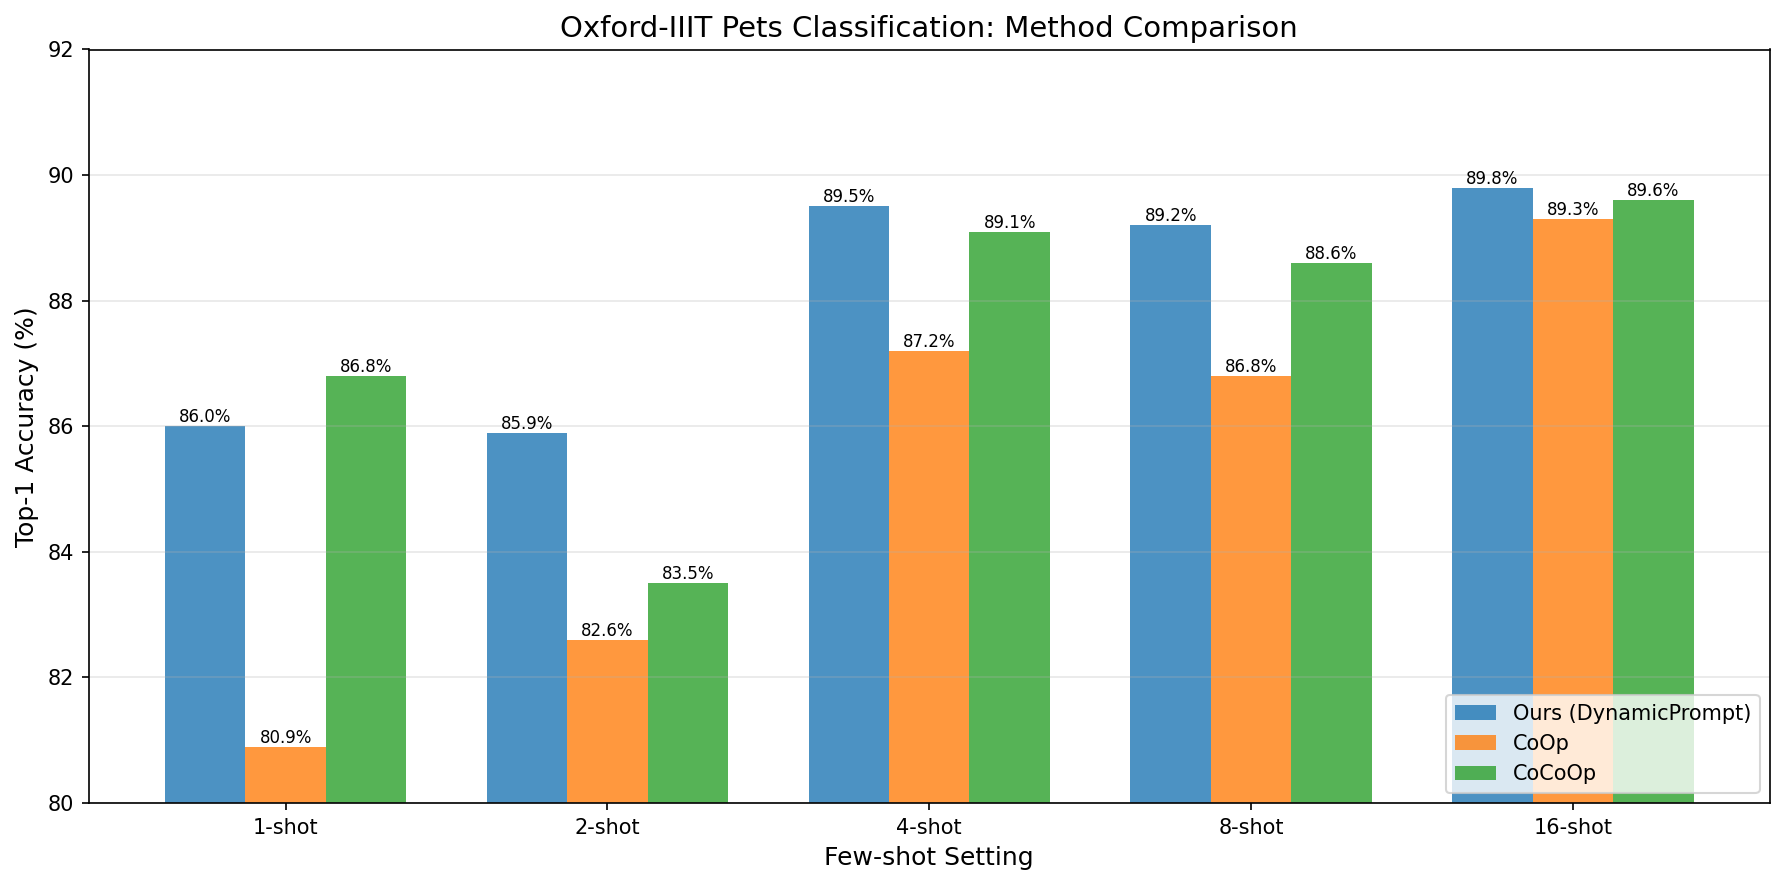
\includegraphics[width=0.82\textwidth]{method_comparison.png}
\caption{不同方法在各 shot 设置下的准确率对比}
\label{fig:method_comparison}
\end{figure}

\begin{figure}[H]
\centering
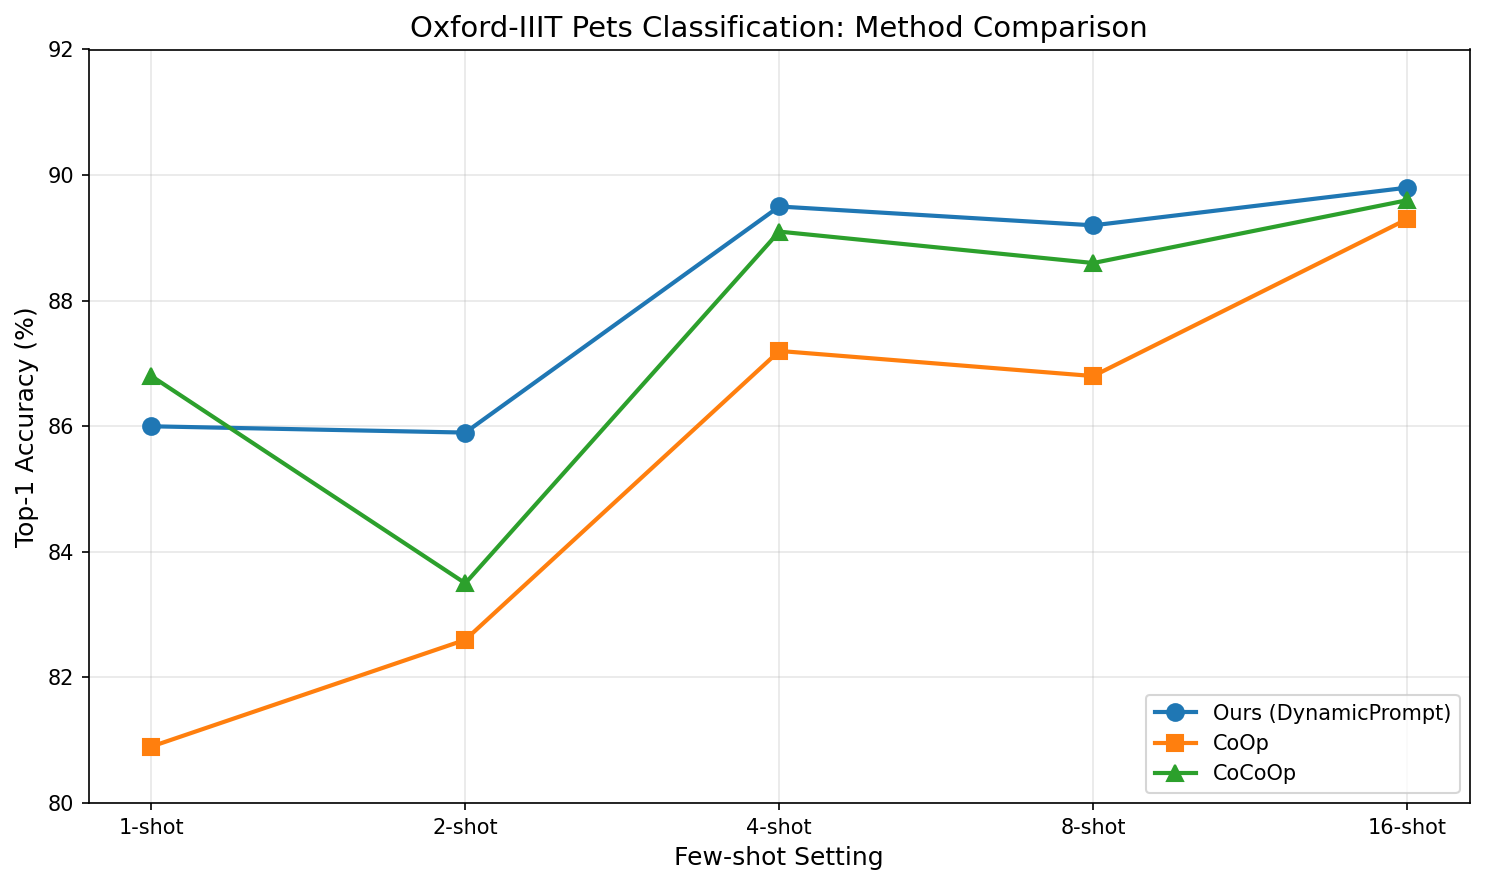
\includegraphics[width=0.82\textwidth]{method_comparison_line.png}
\caption{不同方法准确率随 shot 数变化的趋势}
\label{fig:line_chart}
\end{figure}

进一步观察本文方法与 CoCoOp 的差异可以发现,二者在 4-shot 以后都进入较高精度区间,差距保持在 1 个百分点以内。这表明本文方法并没有通过扩大模型规模来换取提升,而是在样本较少、类别边界尚未稳定时,通过更合理的样本加权获得了更快、更稳的收敛效果。

\subsection{自适应 epoch 策略分析}

图~\ref{fig:adaptive_epochs} 展示了本文最终采用的自适应训练轮数配置。该策略不是额外的模型模块,但对最终结果有实际作用。若直接采用统一 epoch 数,不同 shot 设置下的训练强度并不对等,很难得到稳定比较。将 epoch 数与 shot 数配套后,低样本场景可以获得更充分的迭代,高样本场景则避免了无效训练。

\begin{figure}[H]
\centering
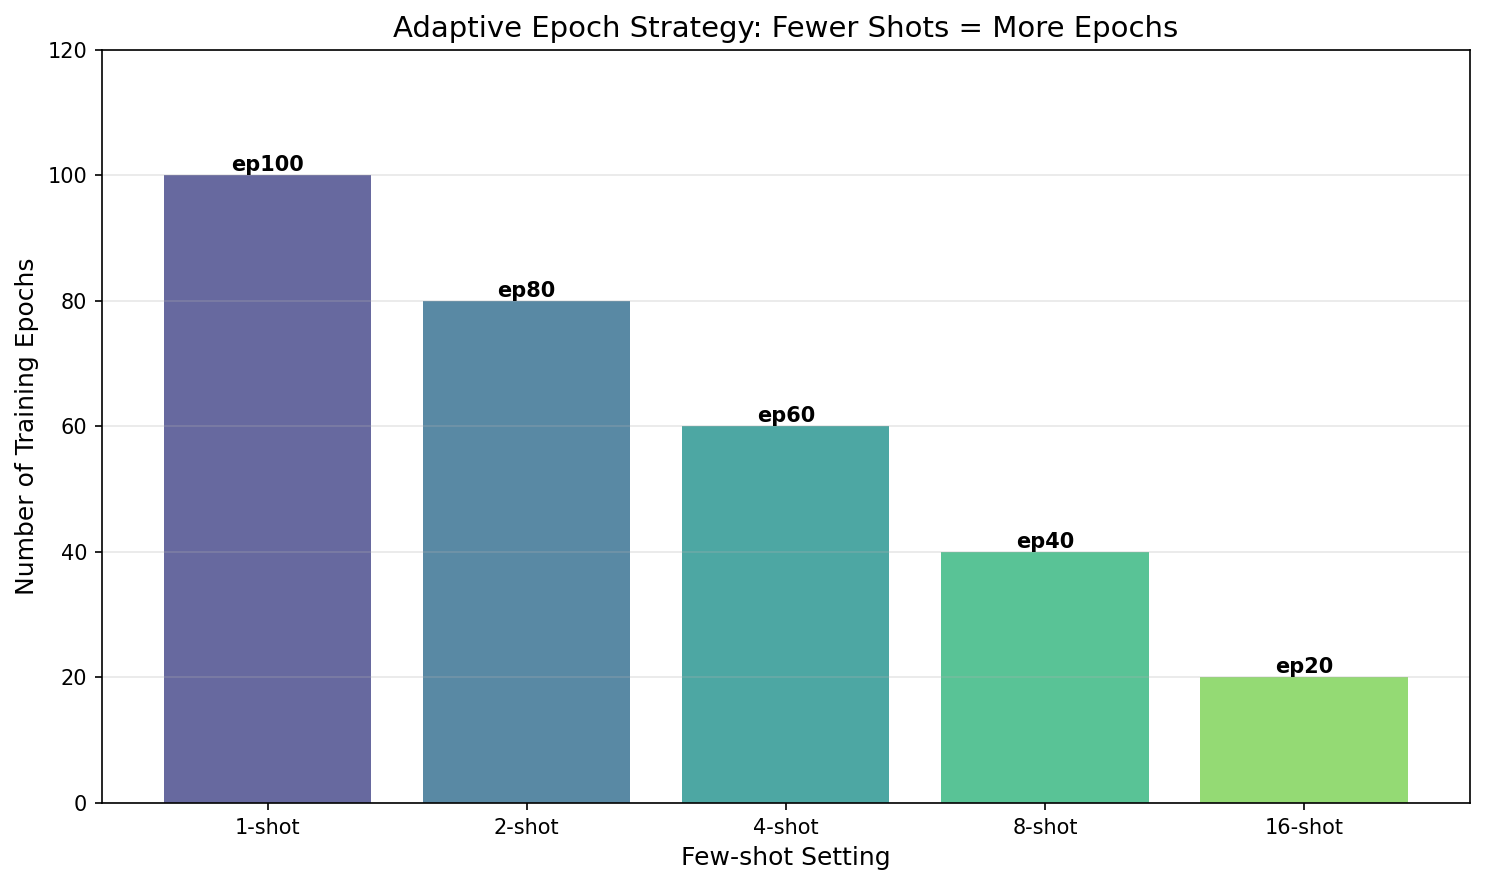
\includegraphics[width=0.68\textwidth]{adaptive_epochs.png}
\caption{不同 shot 设置对应的训练轮数}
\label{fig:adaptive_epochs}
\end{figure}

从最终结果反推,这一策略至少说明两点。第一,本文方法在 2-shot 和 4-shot 下的提升并不是偶然波动,而是在与数据规模匹配的训练轮数下得到的稳定结果。第二,16-shot 虽然只训练 20 个 epoch,仍然达到了 89.8\% 的最佳精度,说明当样本数相对充足时,模型并不依赖长时间训练。

\subsection{与 CoCoOp 的针对性比较}

为了更直观地展示本文方法相对 CoCoOp 的变化,图~\ref{fig:vs_cocoop} 给出了两者在各 shot 设置下的精度差值。可以看到,增益主要集中在 2-shot 到 8-shot 区间,其中 2-shot 的提升最大。这一现象与本文方法的设计目标是一致的: 当样本不足以支撑稳定类别边界时,困难样本权重机制能够帮助模型减少对易分类样本的过度更新,从而把更多训练信号留给边界样本和易混淆样本。

\begin{figure}[H]
\centering
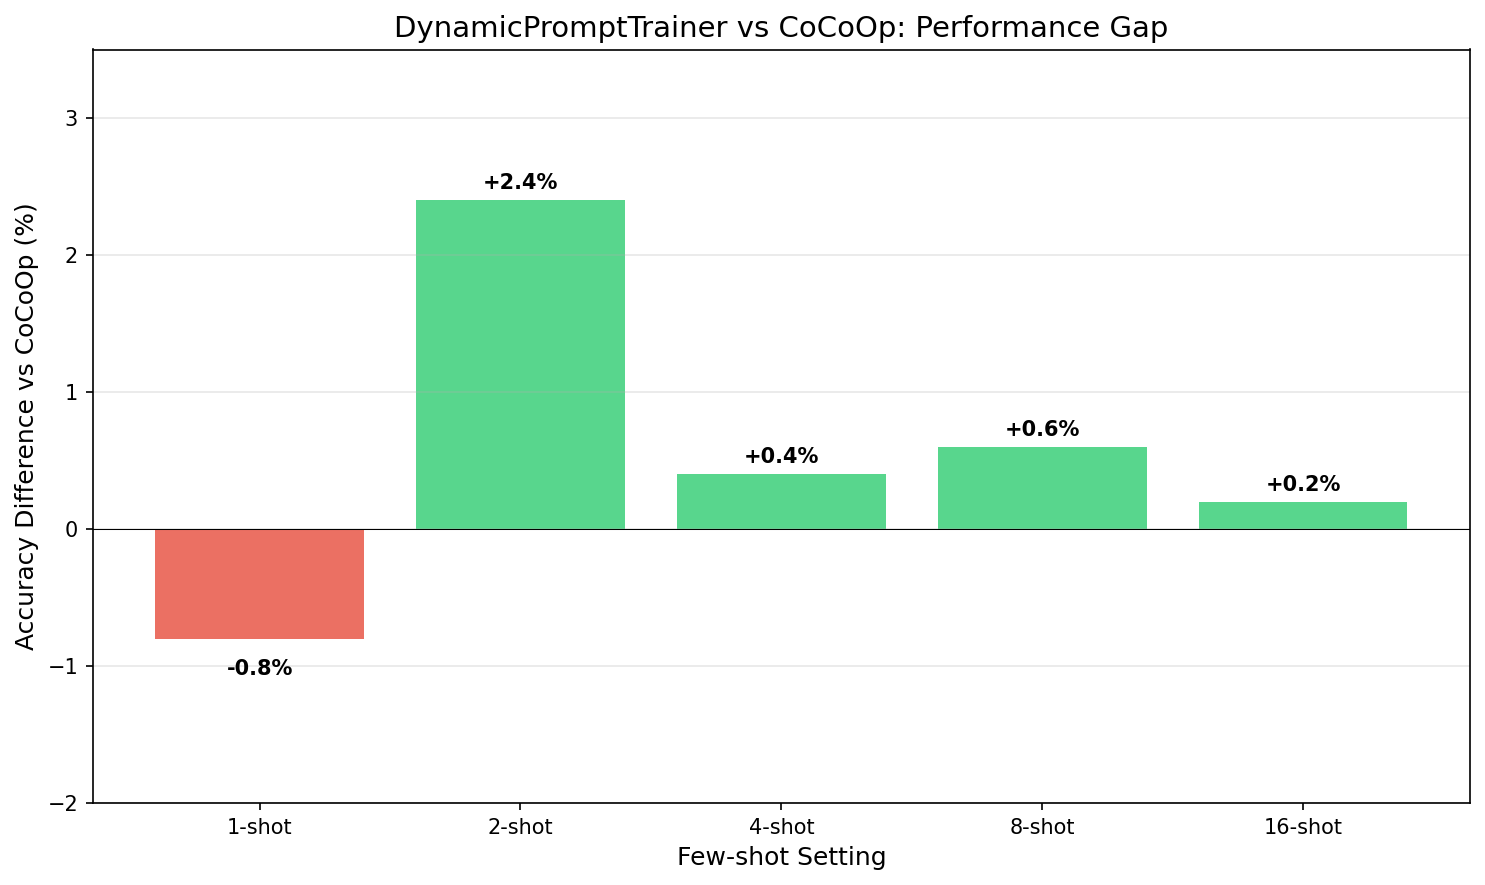
\includegraphics[width=0.68\textwidth]{comparison_vs_cocoop.png}
\caption{DynamicPromptTrainer 相对 CoCoOp 的准确率变化}
\label{fig:vs_cocoop}
\end{figure}

需要说明的是,当前项目中保存了完整的最终对比结果和可视化图表,但没有针对每个单独模块给出独立的消融实验记录。因此本文在这一章不再额外虚构模块拆分结果,而是把分析重点放在已经完成并可核对的主实验结论上。

\section{本章小结}

本章给出了本文方法在 Oxford-IIIT Pets 数据集上的实验设置与结果分析。实验表明,DynamicPromptTrainer 在 2-shot、4-shot、8-shot 和 16-shot 四种设置下均优于 CoCoOp,最高准确率达到 89.8\%。结合图表分析可以看出,本文方法的优势主要体现在小样本到中等样本区间,说明图像条件提示与难度感知加权的结合能够改善 CLIP 在细粒度少样本分类中的训练效果。

\chapter{总结与展望}

\section{全文总结}

本文围绕细粒度猫狗品种识别任务,研究了基于 CLIP 的提示学习方法在少样本条件下的应用问题。针对 CoOp 使用静态提示、CoCoOp 未显式区分样本难度的不足,本文设计并实现了 DynamicPromptTrainer,将图像条件提示生成与难度感知样本加权结合到同一训练框架中。

在方法上,本文完成了以下几项工作。首先,构建 AdaptivePromptLearner,在基础上下文向量之外加入类别自适应因子,使不同类别能够使用不同的提示缩放方式。其次,设计 SoftPromptAdapter,利用两层 MLP 根据图像特征生成提示偏移,让提示词不再固定于单一模板。再次,引入 DifficultyWeightCalculator,根据真实类别预测概率和误分类情况对训练样本赋予不同权重,使困难样本在损失函数中的贡献更大。最后,在原有分类系统之外梳理并整合了推理时安全扩展模块,说明其基于 TTC 的检测与防御机制以及与动态提示模型的集成方式。

在实验上,本文以 Oxford-IIIT Pets 数据集为测试对象,完成了 1-shot、2-shot、4-shot、8-shot 和 16-shot 五组比较实验。结果显示,本文方法在 2-shot、4-shot、8-shot 和 16-shot 设置下均超过 CoCoOp,其中 16-shot 达到 89.8\% 的最高准确率。这说明在细粒度宠物分类任务中,对提示词进行图像条件化调整的同时,再引入面向困难样本的训练权重分配,能够带来稳定收益。

\section{工作不足}

虽然本文方法取得了较好的结果,但当前工作仍有几个明显限制。

第一,实验目前集中在 Oxford-IIIT Pets 单一数据集上,任务类型比较统一。该结果能够说明方法在宠物品种识别上的有效性,但还不足以证明其在鸟类、车型或植物等其他细粒度场景中的泛化能力。

第二,项目中已经完成主实验对比与图表整理,但尚未形成系统的模块级消融实验。例如,单独移除难度权重模块、固定类别自适应因子或替换不同提示初始化方式后的效果,还需要进一步补充。

第三,安全模块虽然已经完成代码集成,并提供了独立评估脚本,但当前本地环境尚未具备完整的数据与依赖条件,因此还没有形成可直接写入论文正文的最终防御实验结果。这意味着安全部分目前主要完成了系统设计与评估流程层面的整理。

\section{后续展望}

后续工作可以从以下几个方面继续推进。

\begin{enumerate}
\item 扩展数据集范围。在保持当前实现框架不变的前提下,将方法迁移到 CUB、Stanford Cars 等细粒度数据集,验证难度感知机制是否具有更普遍的效果。
\item 补充更完整的消融实验。围绕 SoftPromptAdapter、DifficultyWeightCalculator 和类别自适应因子分别开展控制变量实验,进一步解释性能提升来自哪些具体模块。
\item 完善安全评估环境。修正 \texttt{evaluate\_security.py} 中的数据集加载问题,补齐测试数据路径,在统一攻击强度下系统评估防御前后干净样本与对抗样本的准确率变化。
\item 尝试更强的主干网络与提示结构。例如使用 ViT 系列 CLIP 主干,或者探索更长上下文、分层提示和多模板提示的组合方式。
\end{enumerate}

\section{本章小结}

本文完成了一个面向细粒度猫狗分类的动态提示学习系统,并给出了可复现的实验结果。同时,项目还引入了推理阶段的安全扩展模块,为后续开展对抗鲁棒性研究预留了接口。当前工作已经验证了方法的基本有效性,但仍有扩展数据集、完善消融实验和补全安全评估等进一步研究空间。


% -------------------- 参考文献 --------------------
\backmatter
\addcontentsline{toc}{chapter}{参考文献}
\bibliographystyle{plainnat}
\bibliography{ref}

% -------------------- 致谢 --------------------
\chapter*{致谢}
\markboth{致谢}{致谢}
\addcontentsline{toc}{chapter}{致谢}

本科毕业设计从选题、实验到论文整理,前后持续了较长时间。其间我不仅完成了模型实现和实验复现,也逐步体会到把一个看似清晰的想法真正落到代码、数据和结果上,往往比最初预想更细碎,也更考验耐心。

首先感谢指导教师在课题选择、研究思路和论文修改上的持续帮助。每次讨论都不只是指出问题,也让我学会如何把“想做什么”进一步落实为“该怎样验证”。在实验结果不稳定、写作推进缓慢的时候,这些建议对我非常重要。

感谢身边同学在项目实现阶段提供的交流与帮助。无论是训练配置、环境问题,还是论文结构上的讨论,这些及时的反馈都让我少走了不少弯路。

最后感谢家人在整个毕业阶段给予的理解和支持。能够比较完整地完成这项工作,离不开他们在时间、情绪和生活上的包容。


\end{document}
